%%%%%%%%%%%%%%%%%%%%%%%%%%%%%%%%%%%%%%%%%%%%%%%%%%%%%%%%%%%%%%%%%%%%%%
%% Springer Nature LaTeX template (December 2024)                  %%
%% Journal: Public Choice (Springer)                               %%
%% Reference style: sn-basic (author-year via natbib)              %%
%%                                                                 %%
%% Please do not use \input{...} to include other tex files.       %%
%% Submit your LaTeX manuscript as one .tex document.              %%
%%%%%%%%%%%%%%%%%%%%%%%%%%%%%%%%%%%%%%%%%%%%%%%%%%%%%%%%%%%%%%%%%%%%%%

\documentclass[pdflatex,sn-basic]{sn-jnl}

%%%% Standard Packages
\usepackage{graphicx}
\usepackage{multirow}
\usepackage{amsmath,amssymb,amsfonts}
\usepackage{amsthm}
\usepackage{booktabs}
\usepackage{longtable}
\usepackage{tabularx}
\usepackage[skip=1ex]{caption}
\usepackage{subcaption}
\usepackage{adjustbox}
\usepackage{siunitx}
% threeparttable is already loaded by sn-jnl.cls
\usepackage[T1]{fontenc}
\usepackage[english]{babel}
\usepackage{xcolor}
\usepackage{rotating}
\usepackage{setspace}
\usepackage{enumitem}
\usepackage[title]{appendix}
\usepackage{hyperref}

\graphicspath{{../figs/}}

\raggedbottom

\begin{document}

\title[When Pork Changes Hands]{When Pork Changes Hands: Coalition Presidentialism, Legislative Capture, and the Price of Legislative Support in Brazil}

\author*[1]{\fnm{Pedro Caiua} \sur{Campelo Albuquerque}}\email{pedro.caiua@aluno.unb.br}

\author[1,2]{\fnm{Daniel Oliveira} \sur{Cajueiro}}\email{danielcajueiro@unb.br}

\author[1]{\fnm{Rafael Terra} \sur{de Menezes}}\email{rafaelmenezes@unb.br}

\affil*[1]{\orgdiv{Department of Economics}, \orgname{University of Bras\'ilia}, \orgaddress{\street{Campus Universit\'ario Darcy Ribeiro, FACE}, \city{Bras\'ilia}, \postcode{70910-900}, \state{DF}, \country{Brazil}}}

\affil[2]{\orgdiv{National Institute of Science and Technology for Complex Systems (INCT-SC)}, \orgname{University of Bras\'ilia}, \orgaddress{\city{Bras\'ilia}, \postcode{70910-900}, \state{DF}, \country{Brazil}}}

\abstract{Pork-barrel politics has long been the standard explanation for legislative support in coalition-presidential democracies, but the institutional distribution of budget control between the Executive and the Legislature is not static. When constitutional, judicial, or procedural reforms shift control over legislative amendments across institutional actors, the residual margin of bargaining migrates to whichever actor retains procedural control over the budget. Using an instrumental-variables Double Machine Learning strategy on the Brazilian Chamber of Deputies, a paradigmatic case, we document two coefficients that together describe a single phenomenon. First, the canonical pork-for-votes effect on alignment with the Executive reverses sign between consecutive legislatures once the Executive's discretionary leverage over amendment execution is curtailed, turning from positive to negative. Second, the disappearance of the Executive coefficient coincides with the emergence of a positive coefficient on alignment with the Chamber president's party once a new leadership takes office, robust to the exclusion of his own party and absorbed entirely by the broader \emph{Centr\~ao}. The pork-for-votes bargain did not vanish; it changed hands. The residual leverage migrated from the Executive to the Chamber leadership, and the visible-amendment instrument migrated with it. We interpret the regime change as \emph{legislative capture} of the pork channel and argue that the mechanism generalizes: whenever institutional reforms shift control over the budget between principals, the associated bargaining coefficients should be expected to shift with them.}

\keywords{pork-barrel politics, coalition presidentialism, legislative capture, instrumental variables, legislative alignment, Brazil}

\pacs[JEL Classification]{D72, H50, P16}

\maketitle

\footnotetext[1]{Replication code and analysis-ready panel: \href{https://doi.org/10.5281/zenodo.21378905}{doi.org/10.5281/zenodo.21378905}. GitHub repository: \href{https://github.com/pedrocampeloa/pork-votes-brazil}{github.com/pedrocampeloa/pork-votes-brazil}.}

\section{Introduction}
\label{sec:intro}
% ============================================================================

How do executives sustain legislative majorities when their own party commands only a minority of seats? Coalitional presidential systems answer this question with pork: the executive channels federal-budget resources to deputies' districts in exchange for legislative support, and the resulting amendments serve as the principal monetary instrument of coalition management. Brazil has been the empirical laboratory of this argument for nearly four decades. \citet{Abranches1988} coined the term \emph{presidencialismo de coaliz\~ao} to describe how Brazilian presidents assemble broad ideological coalitions through portfolios and pork; \citet{PereiraAndMueller2004} and \citet{Raile2011} provide the foundational evidence that amendment execution causally predicts roll-call alignment with the government. Subsequent work confirms the qualitative pattern \citep{Zucco2009,Power2010,FigueiredoLimongi2000}. The implicit assumption in this literature is that the pork-for-votes relationship is structural, positive, and identified relative to the Executive. We document that none of those three properties holds once the institutional distribution of budget control shifts between principals: the sign is not structural, the direction depends on which actor retains procedural control over the visible amendment, and the identity of the receiving principal is itself endogenous to institutional reform.

Using an instrumental-variables Double Machine Learning (IV-DML) strategy on a panel of $869{,}902$ deputy-vote observations from the 55th and 56th Legislatures, we estimate two coefficients that read together as a single phenomenon. First, the effect of pre-vote amendment commitments on alignment with the Executive is regime-dependent and changes sign between two consecutive legislatures. Under the Rousseff-Temer administrations (Legislature 55, 2015--2018)\footnote{Dilma Rousseff (PT) presided from 1 January 2015 to 31 August 2016, when the Senate concluded her impeachment; Vice-President Michel Temer (MDB) served the remainder of the term through 31 December 2018. We refer to the joint period by the pair to reflect the fact that both governments operated within Legislature 55, and we use ``Temer'' alone in later passages as a shorthand for the coalitional equilibrium that stabilized after the impeachment and produced the pre-2019 pork-for-votes coefficient.}, an additional one million reais of pre-vote committed amendment raises the probability of alignment by $1.73$ percentage points, consistent with the Pereira--Mueller estimate. Under Bolsonaro (Legislature 56, 2019--2022) the same instrument predicts a $0.94$-point \emph{decrease} in Executive alignment, statistically significant at the one-percent level. Second, the disappearance of the Executive coefficient coincides with the emergence of a positive coefficient when the outcome is re-defined as alignment with the formal voting orientation of the party of the Chamber president (the Speaker of the lower house of Congress, elected by his peers and the chief gatekeeper of the legislative agenda). Under the presidency of Rodrigo Maia (DEM, July 2016 through January 2021), pork purchases alignment with DEM in the same direction as alignment with the Temer government, because DEM was a junior member of the Temer coalition. Under the presidency of Arthur Lira (PP, February 2021 onward), the coefficient on alignment with PP is $+0.33$ percentage points per million reais, robust to the exclusion of Lira's own deputies and absorbed entirely by the broader \emph{Centr\~ao} coalition.\footnote{The \emph{Centr\~ao} is a fluid bloc of centrist and center-right parties that trades legislative support for cabinet positions and budget access regardless of who holds the presidency. Its composition varies over time but stabilizes around a set of nine parties (PP, PL, Republicanos, Solidariedade, Uni\~ao Brasil, PTB, Avante, PSD, MDB) in the sample window.}

The two coefficients organize into a single substantive thesis. The pork-for-votes bargain did not stop functioning under Bolsonaro. The bargain changed hands. Under the programmatic-coalitional regime of the Temer presidency, an Executive bargaining with a fragmented multiparty coalition allocated visible amendments along a loyalty gradient documented by the classical literature \citep{PereiraAndMueller2004,Raile2011}. Under the Bolsonaro presidency, the same allocation device produced a negative coefficient in the Executive-aligned outcome and a positive coefficient of comparable order of magnitude in the outcome aligned with the new Centr\~ao-led Chamber leadership. We refer to this institutional transfer as \emph{legislative capture} of the pork channel. The empirical reversal is not a vanishing of distributive bargaining but a re-routing through a different institutional principal, conditioned by the constitutional changes that bound the Executive's discretionary leverage between 2015 and 2019 and completed by the election of an opposition Chamber president in February 2021.

Establishing causality requires a strategy that survives the well-known endogeneity of pork allocation. The Executive observes deputies' reservation prices and allocates resources strategically, so naive regressions confound the structural effect with the allocation rule \citep{BerryGrosscloseMilyo2000,DesposatoCOE2006}. We instrument amendment commitments with the \emph{ministry execution backlog}, a deputy-specific shock rooted in the administrative capacity of the ministry through which each deputy's amendment is processed. Ministries enter each fiscal year with zero year-to-date execution and build up gradually; a ministry entering the fourth quarter with a low cumulative execution rate faces acute administrative pressure to commit funds before the December~31 expiration deadline established by Article~35 of the 1964 Budget Law. Deputies whose amendments flow through such ministries receive an exogenous acceleration of commitments driven by administrative backlog clearing, not by the political value of any specific vote. The instrument's identifying variation is cross-deputy heterogeneity in the ministry-level cumulative execution rate, conditional on bill-type, thematic, and electoral-cycle controls; the December~31 deadline supplies the mechanism but is not itself the exclusion-satisfying variation. The first-stage $F$-statistic exceeds $4{,}000$ in each legislature separately, well above the Stock--Yogo critical value of $10$ \citep{StockYogo2005}. We fold this instrument into a partially-linear IV framework with high-dimensional non-parametric controls \citep{Chernozhukov2018}, deputy and party fixed effects, and cluster-robust standard errors.

A natural alternative interpretation of the negative Executive-aligned coefficient must be confronted explicitly. Between 2020 and 2022 the Bolsonaro government routed an estimated R\$45 billion through rapporteur amendments, classified RP-9 in the budget nomenclature, a category of transfers operating outside the standard transparency requirements. The Brazilian Supreme Court (STF, the apex constitutional court) issued a preliminary injunction against the mechanism in November 2021 and declared it unconstitutional in December 2022, after which the political function of the opaque channel migrated to committee (RP-8) and Pix amendments (a direct-deposit modality established by EC 105/2019). Because RP-9 transfers were not individually attributable to deputies during the period of operation, our treatment variable measures only visible amendments, and the Bolsonaro-era coefficient mechanically understates the total pork-for-votes effect through opaque channels. We treat this as a limitation on the \emph{magnitude} of the negative coefficient rather than as a competing interpretation of its sign or of the legislative-capture finding. The opaque channel is, in our reading, the third leg of the same institutional transfer documented in the visible-amendment evidence: nominal authorship of RP-9 was assigned to the budget rapporteur, an institutional figure named by the Chamber president, and the post-2022 RP-8 substitution preserved the legislative authorship structure.

The paper makes three contributions. First, to the literature on pork-barrel politics and coalition presidentialism, we show that the positive sign of the classical pork-for-votes coefficient is not invariant. The Temer-era estimate replicates the classical \citet{PereiraAndMueller2004} pattern; the Bolsonaro-era estimate reverses it. To our knowledge, this is the first documentation of a sign reversal in the Brazilian pork-for-votes relationship within a continuous panel. Second, we document that the sign reversal is conditional on the institutional identity of the principal. When the outcome is re-defined to track the Chamber president's party rather than the Executive's, the Bolsonaro-era coefficient turns positive, and the regime change is best read as a transfer of bargaining authority across institutional actors rather than as a vanishing of the bargaining technology. Third, methodologically, we document that the choice of inter-annual fixed effects in IV-DML estimation can be consequential when the instrument extracts inter-annual variation. We make this trade-off explicit in our preferred specification and treat it as a feature of what the instrument identifies rather than as a discretionary modeling choice.

The remainder of the paper is organized as follows. Section~\ref{sec:institutional} describes the institutional setting, including the legal architecture, the RP-9 episode, the year-end execution calendar, and the aggregate stylized facts. Section~\ref{sec:data} describes the data. Section~\ref{sec:strategy} presents the IV-DML strategy. Section~\ref{sec:results} reports the two central results: the sign reversal in Executive alignment (Subsection~\ref{subsec:main_gov}) and the alignment with the Chamber president (Subsection~\ref{subsec:legislative_capture}). Section~\ref{sec:discussion} interprets the regime change and discusses limitations. Section~\ref{sec:conclusion} concludes. Robustness exercises are in Appendix~\ref{app:robustness}.

% ============================================================================
\section{Institutional setting}
\label{sec:institutional}
% ============================================================================

Brazil's political system combines a multiparty fragmented legislature, in which the 56th Chamber seated representatives from 30 parties, with a strong executive legislative agenda \citep{Abranches1988,FigueiredoLimongi2000}. Each federal deputy is constitutionally entitled to designate a portion of the federal budget for projects in her electoral district. The Brazilian federal budget recognizes four categories of parliamentary amendment, identified by primary-result code: individual amendments (RP-6), state-bench amendments (RP-7), committee amendments (RP-8), and rapporteur amendments (RP-9). The categories differ in authorship, statutory cap, and, of more direct relevance for our identification, in whether the Executive retains discretion over their execution. The composition of total amendment spending across the four categories has shifted substantially over the past decade. These shifts originated in constitutional amendments, in a Supreme Court ruling, and in the annual Budget Directives Law, and are therefore exogenous to any individual deputy's bargaining position.

\subsection{The legal architecture of mandatory execution}
\label{subsec:legal_architecture}

Constitutional Amendment 86 of 2015 marked the end of the long period during which the Executive retained broad discretion over the execution of parliamentary amendments. Until then, discretionary execution operated as a continuous bargaining instrument: \citet{PereiraAndMueller2004} document how cabinet portfolios and amendment execution jointly predicted legislative alignment in pre-2015 data, and \citet{Raile2011} shows that the optimal mix of pork, portfolios, and ideology shapes coalition stability. Three constitutional amendments and one Supreme Court intervention between 2015 and 2022 reshaped this legal architecture. EC 86 of 2015 made individual amendments (RP-6) mandatory up to 1.2 percent of net current revenue (RCL, the reference base for federal fiscal ceilings), with half of the obligation reserved for the health sector. Execution rates for individual amendments rose accordingly, exceeding 90 percent in every year since 2016 against pre-2015 averages near 30 percent. EC 100 of 2019 extended mandatory execution to state-bench amendments (RP-7) up to 1 percent of RCL, in effect from the 2020 budget cycle onward. EC 105 of 2019 introduced a new transfer mode within RP-6 known as ``Pix amendments,'' which deliver resources directly from the Federal Treasury to municipalities or states without an intermediate state-level contract; the modality reduces administrative friction at the cost of ex-post traceability. The cumulative effect of the three amendments was to remove the volume of mandatory amendments from the Executive's discretionary toolkit. The residual margin of bargaining shifted toward the timing of execution and the choice of modality. Intra-year timing is the margin our identification exploits.

Table~\ref{tab:rp_legal_status} summarizes the five amendment categories and their legal status before and after the post-2015 reforms. Three of the five categories (RP-6, RP-6 Pix, RP-7) underwent a discrete transition from Executive-discretionary to constitutionally mandatory execution between 2015 and 2020; the remaining two (RP-8, RP-9) preserved their discretionary status until RP-9 was extinguished by the STF's ADPF 854 ruling in 2022 (a constitutional challenge filed before the Supreme Court). The substantive content of the reform is that the volume dimension of pork allocation passed from the Executive to constitutional mandate, while the timing dimension (the within-year scheduling of commitments and payments) remained under Executive control and provides the source of exogenous variation our instrument exploits.

\begin{table}[htbp]
\centering
\caption{Parliamentary amendment categories: legal status before and after the post-2015 reforms.}
\label{tab:rp_legal_status}
\small
\setlength{\tabcolsep}{5pt}
\begin{tabular}{@{}lllll@{}}
\toprule
Code & Authorship              & Pre-2015        & Post-reform status \\
\midrule
RP-6     & Individual deputy       & Discretionary   & \textbf{Mandatory} (from 2015) \\
RP-6 Pix & Individual deputy       & Did not exist   & \textbf{Mandatory} (from 2020) \\
RP-7     & State-bench (collective)& Discretionary   & \textbf{Mandatory} (from 2020) \\
RP-8     & Standing committee      & Discretionary   & Discretionary \\
RP-9     & Budget rapporteur       & Discretionary   & Discretionary (until 2022) \\
\bottomrule
\end{tabular}
\begin{tablenotes}
\small
\item Notes: ``RP'' refers to the primary-result code in the federal budget nomenclature, which classifies expenditure by its institutional origin and execution rule. Mandatory amendments must be executed by the Executive up to the constitutional ceiling indicated; discretionary amendments may be executed or withheld at the Executive's choice within the year. Our treatment variable in the IV-DML specification (Sections~\ref{sec:data}--\ref{sec:strategy}) is the pre-vote committed value of RP-6 amendments to the deputy in question, the channel for which deputy-level authorship is unambiguous throughout the sample window; the remaining categories appear in the institutional discussion of Section~\ref{sec:institutional} and in the alternative outcomes of Section~\ref{sec:results}.
\end{tablenotes}
\end{table}

\subsection{The RP-9 episode and its substitution}
\label{subsec:rp9_episode}

The consolidation of the rapporteur channel had a political counterpart. Facing a fragmented Chamber and rising impeachment pressure through 2020, the Bolsonaro government had to secure the February 2021 Chamber-presidency election against Baleia Rossi (MDB), the candidate endorsed by outgoing Chamber president Rodrigo Maia in December 2020. Bolsonaro backed Arthur Lira (PP), who won the plenary vote on 1 February 2021 by 302 to 145, and the Centr\~ao became the pivotal legislative bloc for the remainder of the administration. The alignment operated as an implicit exchange: the Executive ceded a share of budget-execution control to the legislative leadership in return for governability and protection against impeachment votes on the floor \citep{GrazianeEtAl2022RP9,BrazilReports2022SecretBudget}. The formalization of RP-9 in the 2020 Budget Directives Law and its rapid expansion in the following years \citep{TCU2022RelatorioContas} were the visible fiscal imprint of this exchange, along with the migration of cabinet appointments into Centr\~ao hands. The regime change we document is therefore not only a passive reflection of the post-2015 constitutional constraints on Executive discretion; it was actively negotiated between the Executive and the Chamber leadership in the 2020--2022 window.

Between 2020 and 2022 the Bolsonaro government routed an estimated R\$45 billion in committed value through rapporteur amendments classified under primary-result code RP-9. Although the line had existed since 2016 with negligible volume, the 2020 Budget Directives Law (LDO 2020) consolidated RP-9 as the principal channel of executive-legislative bargaining: R\$21.2 billion in 2020, R\$16.7 billion in 2021, and R\$8.6 billion in 2022. RP-9 transfers were nominally attributed to the budget rapporteur rather than to individual deputies. The actual political authorship was registered only as a list of supporting parliamentarians, with limited public disclosure and no individual identification in the official budget data during the period of operation. The Supreme Court issued a preliminary injunction (ADPF 854) demanding partial disclosure in November 2021 and declared the mechanism unconstitutional in December 2022. RP-9 was formally extinguished in the 2023 budget.

The substitution dynamics that followed the STF ruling are quantitatively pronounced. Committee amendments (RP-8), which had averaged below R\$0.6 billion per year between 2016 and 2022, grew to R\$6.9 billion in 2023 and R\$11.7 billion in 2024, a roughly twentyfold increase concentrated in the two years immediately following the extinction of RP-9. Pix amendments under EC 105 followed a parallel trajectory, growing from R\$3.3 billion in 2022 to R\$7.7 billion in 2024. The combined volume of RP-8 and Pix amendments in 2023 and 2024 closely tracks the volume of RP-9 in 2020 through 2022, indicating that the political function of the opaque transfer channel survived the institutional intervention through relabeling rather than through a substantive reduction in opacity. A joint technical note from Transpar\^encia Brasil, Transpar\^encia Internacional Brasil, and Contas Abertas filed with the STF in September 2025 documents continued violations of the disclosure requirements imposed by ADPF 854 \citep{TransparenciaBrasil2025}. The 57th Legislature falls outside the sample window: the corresponding term is still in progress and the deputy-level execution data are not yet available with the same coverage. The RP-9 episode has two consequences for the analysis that follows. Because RP-9 was not individually attributable to deputies during the period of operation, our treatment variable measures only visible amendments, and the Bolsonaro-era coefficient is mechanically incomplete. The existence of an opaque parallel mechanism, and its post-ADPF 854 reincarnation through RP-8 and Pix amendments, is itself a constitutive feature of the institutional regime change that conditions the sign of the pork-for-votes coefficient.

\subsection{The year-end execution cycle and the identification window}
\label{subsec:execution_cycle}

The empirical core of our identification is the year-end commitment cycle. Brazilian federal expenditure follows three legal stages under Law 4.320/1964 \citep{Lei4320}: commitment (the formal reservation of funds, which creates a legal payment obligation), settlement (verification that the contracted party fulfilled its obligations), and payment (the cash transfer itself). Article 35 establishes that appropriations not committed by December 31 permanently expire; the spending authority lapses and funds return to the National Treasury. The government does not ``return'' money in any active sense; the authorization simply ceases to exist. To preserve a deputy's amendment within the fiscal year the government must register the commitment before midnight on December 31, and four institutional mechanisms make this near-mandatory. The constitutional obligation introduced by EC 86/2015 means non-execution is now legally actionable; deputies can seek writs of mandamus before the STF, and ministers can face liability under Law 1.079/1950. Bureaucratic ``use-it-or-lose-it'' pressure from the Federal Budget Secretariat reduces ministries' baselines in the following year's budget process. Real-time deputy monitoring via the Federal Transparency Portal generates immediate political friction from any uncommitted amendment. And the carry-over appropriations mechanism allows commitments to be preserved into the following year even when settlement is incomplete, removing any cash-flow justification for non-commitment. The result is a sharp December commitment spike that is administratively, not politically, driven.

Figure~\ref{fig:seasonality} illustrates the resulting calendar mismatch. Voting activity peaks in May, when the legislative agenda is heaviest. Amendment commitments peak in December, when plenary activity is winding down before recess. December alone concentrates $25.0$ percent of annual commitment value while housing only $12.1$ percent of roll-call votes; the Q4 commitment-to-vote ratio is $1.45$, against $1.20$ in Q2 and $0.79$ in Q3. This systematic mismatch between the two calendars is precisely what makes the fiscal deadline an exogenous instrument: the government's incentive to register commitments in December is driven by the Treasury's programming calendar, not by the political value of any specific vote scheduled that month.

\begin{figure}[htbp]
\centering
\includegraphics[width=0.78\textwidth]{fig_seasonality.pdf}
\caption{Monthly distribution of parliamentary amendment commitments (bars, left axis) versus roll-call votes (line, right axis), Legislatures 55--56 (2016--2022). The two calendars are misaligned: voting peaks in May ($16.5$\% of annual votes) while amendment commitments peak in December ($25.0$\%, driven by the Article 35 year-end deadline). Commitments restricted to deputy-attributable individual and state-bench amendments (RP-6 + RP-7) processed through the SICONV/Transferegov system. This institutional misalignment, with amendment commitments concentrated at year-end for administrative reasons and votes distributed across the year for political ones, supplies the deputy-specific administrative pressure that our instrument exploits.}
\label{fig:seasonality}
\end{figure}

\subsection{Aggregate stylized facts}
\label{subsec:stylized_facts}

The institutional shifts described above translate into three aggregate patterns: a sharp increase in the total volume of amendments between 2014 and 2025, a recomposition of channel shares across the four primary-result categories, and a deputy-level pivot in 2020 through 2022 between visible individual amendments and the opaque rapporteur channel. The patterns are computed from the consolidated amendment data published by the Federal Transparency Portal \citep{ControladoriaGeralDaUniao2026} and the Federal Treasury's RGF reports.

Table~\ref{tab:stylized} reports the year-by-modality breakdown together with the share of total amendments in federal primary discretionary spending. The denominator measures the slice of the budget the Executive can actually reallocate, after excluding rigid items such as debt service, pensions, civil-service payroll, and constitutional transfers; it captures the universe over which institutional bargaining can take place. Total amendment commitments rose from $5.1$ percent of discretionary spending in 2014 to $26.9$ percent in 2025, a 5.3-fold increase that captures both the rising volume of amendments and the corresponding contraction of the Executive's free fiscal space. Two further columns of the table decompose the post-2019 share into a mandatory channel (RP-6 plus RP-7, subject to compulsory execution under EC 86/2015 and EC 100/2019) and an Executive-discretionary residual (RP-8 plus RP-9). The mandatory channel rises from $9.9$ percent of discretionary spending in 2019 to $20.5$ percent in 2025, while the discretionary residual peaks at $12.9$ percent in 2020 under the Secret Budget regime (the colloquial label for the rapporteur-amendment channel that operated 2020--2022 without individual attribution) and falls to $6.4$ percent by 2025 after the STF intervention. Total amendments grew from R\$6.1 billion in 2014 to R\$47.1 billion in 2025 in nominal terms, a 670 percent increase against a cumulative inflation of approximately 85 percent. Measured against the broader denominator of Net Current Revenue (the legal reference for the EC 86/2015 ceiling of 1.2 percent of RCL), the same series grew from $0.95$ percent to $3.25$ percent over the window. Figure~\ref{fig:composition} represents the recomposition as two stacked-area panels sharing the same horizontal axis: the top panel decomposes the annual total by primary-result category and reports the share of federal discretionary spending on the right axis, and the bottom panel decomposes the same total by legal status.

\begin{table}[htbp]
\centering
\caption{Annual amendment commitment by primary-result category, 2014--2025.}
\label{tab:stylized}
\small
\setlength{\tabcolsep}{4pt}
\begin{tabular}{lrrrrrrrrr}
\toprule
& \multicolumn{5}{c}{Amendment value (R\$ bi)} & & \multicolumn{3}{c}{Share of discretionary spending (\%)} \\
\cmidrule(lr){2-6} \cmidrule(lr){8-10}
Year & RP-6 & RP-6 Pix & RP-7 & RP-8 & RP-9 & Total & Total & Mandatory & Discr.\\
\midrule
2014 & 6.1  & --    & --    & --    & --    & 6.1  & 5.1  & --   & --   \\
2015 & 3.4  & --    & --    & --    & --    & 3.4  & 2.9  & --   & --   \\
2016 & 7.2  & --    & 3.6   & 1.3   & 13.7  & 25.9 & 20.9 & --   & --   \\
2017 & 7.1  & --    & 5.1   & 0.9   & 4.5   & 17.5 & 14.0 & --   & --   \\
2018 & 8.5  & --    & 3.4   & 0.2   & --    & 12.0 & 9.2  & --   & --   \\
2019 & 8.5  & --    & 4.7   & 0.2   & 0.4   & 13.9 & 10.3 & 9.9  & 0.5  \\
2020 & 8.6  & 0.6   & 6.5   & 0.6   & 21.2  & 37.5 & 22.3 & 9.3  & 12.9 \\
2021 & 7.4  & 2.0   & 7.2   & --    & 16.7  & 33.4 & 24.8 & 12.4 & 12.4 \\
2022 & 7.4  & 3.3   & 5.8   & 0.3   & 8.6   & 25.5 & 13.1 & 8.5  & 4.6  \\
2023 & 13.8 & 7.1   & 7.6   & 6.9   & --    & 35.4 & 20.2 & 16.3 & 3.9  \\
2024 & 17.0 & 7.7   & 8.4   & 11.7  & --    & 44.8 & 26.7 & 19.7 & 7.0  \\
2025 & 17.3 & 7.0   & 11.6  & 11.2  & --    & 47.1 & 26.9 & 20.5 & 6.4  \\
\midrule
\multicolumn{6}{l}{\emph{Change 2014--2025}} & $+672\%$ & $\times 5.3$ & \multicolumn{2}{c}{see narrative} \\
\bottomrule
\end{tabular}
\begin{tablenotes}
\small
\item Notes: Values in the first six numeric columns are committed amendment volumes in R\$ billions, nominal. ``RP-6 Pix'' is the EC 105/2019 transfer modality (a subset of RP-6), reported separately for transparency. The three ``Share of discretionary spending'' columns report the ratio of amendment commitments to federal primary discretionary spending (the IFI-NT57 / Tesouro Transparente definition of the residual budget the Executive can reallocate after mandatory items). ``Total'' is all amendments; ``Mandatory'' counts RP-6 plus RP-7 (subject to compulsory execution under EC 86/2015 and EC 100/2019, the latter binding from the 2020 budget); ``Discr.''\ counts RP-8 plus RP-9. The mandatory/discretionary split is reported from 2019 onward, when RP-7 began the transition to mandatory status. Dashes denote categories with negligible or zero committed value.
\end{tablenotes}
\end{table}

\begin{figure}[htbp]
\centering
\includegraphics[width=\textwidth]{fig_composition.pdf}
\caption{Composition of parliamentary amendments, 2014--2025. Panel (a) breaks the annual total into the five primary-result categories and overlays, on the right axis, the share of total amendments in federal discretionary primary spending (dashed teal line); Panel (b) breaks the same total into the two legal-status classes. The two panels share the horizontal axis, so the stacked height at any year corresponds to the same annual total; only the internal partition differs. Both panels use committed values in R\$ billions, nominal. In panel (b), the blue area (Mandatory) absorbs each RP the year its constitutional reform enters into force: RP-6 in 2015 (EC 86/2015), RP-6 Pix in 2020 (EC 105/2019), and RP-7 in 2020 (EC 100/2019); the hatched red area (Discretionary) contains the pre-reform years of those RPs plus RP-8 and RP-9 throughout. Vertical dashed lines mark the institutional events that conditioned the trajectory: EC 86/2015, EC 100 and EC 105/2019, the 2020 expansion of the rapporteur channel, the election of Arthur Lira as Chamber president in February 2021, the STF preliminary injunction of November 2021, and the ADPF 854 final ruling.}
\label{fig:composition}
\end{figure}

The third pattern relevant to our analysis is the structural separation between the Centr\~ao bloc and the rest of the Chamber, and its sharpening after the election of Arthur Lira as Chamber president in February 2021. We define the Centr\~ao as the standard nine-party cluster (PP, PL, Republicanos, Solidariedade, Uni\~ao Brasil, PTB, Avante, PSD, MDB), following the categorization used by \citet{Power2010}. The Centr\~ao accounts for $19.8$ percent of the deputy-vote observations in Legislature 55 and $41.8$ percent in Legislature 56, a near doubling that reflects the absorption of the bulk of the Bolsonaro coalition into the bloc after the dissolution of the original PSL-led core in mid-2020. Table~\ref{tab:centrao_descriptive} reports mean alignment with the government and with the party of the Chamber president, plus mean amendment allocation, across the Centr\~ao and non-Centr\~ao groups, separated by sub-period of Legislature 56. The Centr\~ao maintains alignment with the Executive above $0.89$ throughout the legislature, against alignment of $0.61$ to $0.65$ in the non-Centr\~ao. The pattern shifts when we look at alignment with the Chamber president's party. Within the Centr\~ao, alignment with the Chamber-president party rises from $0.902$ pre-Lira to $0.929$ post-Lira while alignment with the Executive falls from $0.912$ to $0.898$ over the same window; in the post-Lira sub-period the Centr\~ao is more aligned with the Chamber-president party than with the Executive. The Pix share of total RP-6 also jumps from approximately $4$ percent before the Lira election to $20.7$ percent (non-Centr\~ao) and $24.5$ percent (Centr\~ao) afterward, with the Centr\~ao preferring the less traceable modality at a noticeably higher rate. Mean RP-6 allocation in volume terms is close to identical across the two groups.

\begin{table}[htbp]
\centering
\caption{Mean alignment and amendment allocation by Centr\~ao status and sub-period (Legislature 56).}
\label{tab:centrao_descriptive}
\small
\setlength{\tabcolsep}{6pt}
\begin{tabular}{lcccc}
\toprule
& \multicolumn{2}{c}{Non-Centr\~ao} & \multicolumn{2}{c}{Centr\~ao} \\
\cmidrule(lr){2-3}\cmidrule(lr){4-5}
& Pre-Lira & Post-Lira & Pre-Lira & Post-Lira \\
\midrule
$N$ obs.                              & 145{,}686 & 228{,}657 &  91{,}259 & 177{,}992 \\
Mean alignment with Executive         & 0.655 & 0.610 & 0.912 & 0.898 \\
Mean alignment with Chamber president & 0.670 & 0.633 & 0.902 & 0.929 \\
RP-6 (R\$M, per obs.)                  & 2.203 & 2.382 & 2.306 & 2.245 \\
Pix (R\$M, per obs.)                   & 0.085 & 0.623 & 0.095 & 0.728 \\
Pix / RP-6 (\%)                       & 3.7   & 20.7  & 4.0   & 24.5  \\
\bottomrule
\end{tabular}
\begin{tablenotes}
\small
\item Notes: Pre-Lira and Post-Lira denote the sub-periods of Legislature 56 separated by the election of Arthur Lira (PP) as Chamber president on 1 February 2021. Mean alignment with Executive is the within-period mean of $y_{it}^{\mathrm{gov}} = \mathbb{1}\{\text{vote}_{it} = \text{government orientation}\}$; mean alignment with Chamber president is the analogous statistic for $y_{it}^{\mathrm{pres}} = \mathbb{1}\{\text{vote}_{it} = \text{orientation of the Chamber president's party}\}$, computed on the subset of observations for which the Chamber-president orientation is recorded (95\% coverage under Maia, 66\% under Lira). Amendment values are per-deputy-vote-window means of pre-vote 60-day committed amount in R\$ millions. The Pix / RP-6 row reports the share of Pix amendments in the total of individual amendments, in percent.
\end{tablenotes}
\end{table}

\subsection{The polarization environment of the sample window}
\label{subsec:polarization_context}

The 55th and 56th Legislatures spanned two markedly different phases of legislative polarization. Because part of the interpretation that follows relies on the reader's mental image of the political environment in which the bargains we study took place, we document that environment directly from the roll-call data. Figure~\ref{fig:polarization_backdrop} plots two simple descriptive measures for every year of the sample. The first is the mean absolute gap between the share of coalition deputies voting ``Yes'' and the share of opposition deputies voting ``Yes,'' averaged across all substantive roll-calls in the year; the second is the share of substantive roll-calls that meet a $70/30$ polarization threshold, defined as one of the two sides voting ``Yes'' at a rate of at least $70\%$ while the other side does so at a rate of at most $30\%$, or vice versa. Both statistics depend only on the vote outcome and on the coalition-opposition classification already used in the paper's dependent variable, so they can be replicated from the raw panel without any external construction.

\begin{figure}[htbp]
\centering
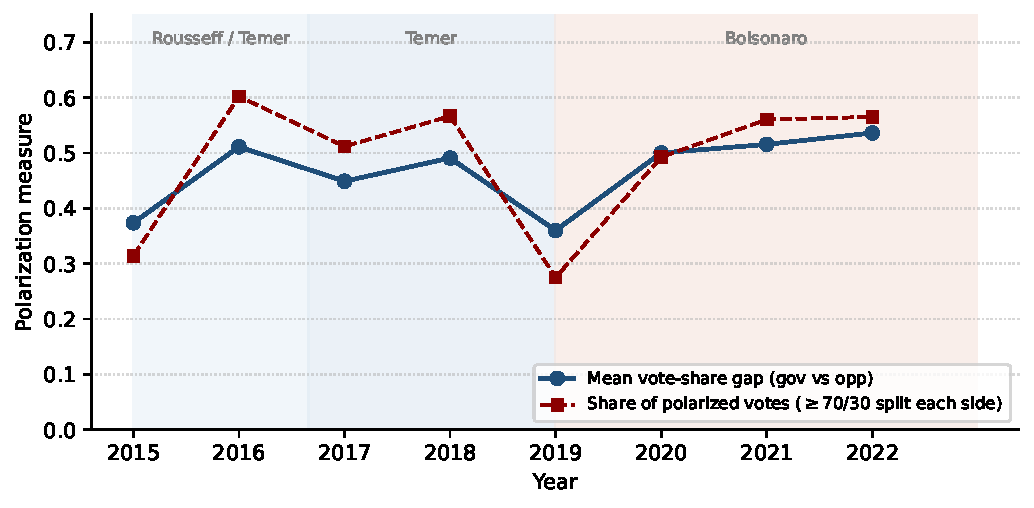
\includegraphics[width=0.8\textwidth]{fig_polarization_backdrop.pdf}
\caption{Legislative polarization environment during the sample window. Blue line and left axis: mean absolute gap between coalition and opposition shares voting ``Yes'' across all substantive roll-calls in the year. Red dashed line: annual share of substantive roll-calls meeting the $70/30$ threshold (see text). Shaded regions indicate presidential sub-periods. The 2016 spike coincides with the Rousseff impeachment vote. The 2019 dip captures the honeymoon of the incoming Bolsonaro administration; the plateau from 2020 onward describes the post-honeymoon regime in which our Legislature 56 results are identified.}
\label{fig:polarization_backdrop}
\end{figure}

The pattern the figure describes is the empirical backdrop for the results that follow. The 2016 impeachment period registers as a peak in both measures. The Temer administration operates in a moderately polarized environment. The Bolsonaro first year exhibits an unusual dip, consistent with the government's initial honeymoon, followed by a return to a persistently more polarized regime from 2020 onward, which is the regime that dominates the Legislature 56 sample by observation count. We make no causal claim about the relationship between this trajectory and the coefficients estimated in Section~\ref{sec:results}. The measure is not used as a mediator, moderator, or control in any of the specifications reported below. Its purpose is only to make explicit the legislative environment in which the two regime-specific coefficients were identified.

% ============================================================================
\section{Data}
\label{sec:data}
% ============================================================================

Roll-call vote data come from the Chamber of Deputies Open Data API.\footnote{\url{https://dadosabertos.camara.leg.br}.} We retain votes where the government leadership issued a directional orientation (``yes'' or ``no''), excluding free-vote releases. Bill types included are constitutional amendments (PEC), provisional measures (MPV), complementary laws (PLP), and ordinary laws (PL) under urgency or priority regimes. The sample spans the 55th and 56th Legislatures (February 2015 to December 2022) and contains $869{,}902$ deputy-vote observations corresponding to 931 unique deputies, with $226{,}308$ observations in Legislature 55 and $643{,}594$ in Legislature 56. The dependent variable equals one when the deputy's vote matches the government's stated orientation and zero otherwise; sample mean alignment is $0.74$.

Amendment commitment data come from the Federal Transparency Portal. Our treatment variable measures total committed amendment value, in millions of reais and winsorized at the 99th percentile, credited to the deputy in a 60-day pre-vote window. We use the left (pre-vote) window as the main specification because forward-looking bargaining theory predicts the pre-vote channel should dominate \citep{Raile2011}; a symmetric $\pm 45$-day window is reported as robustness. The treatment has substantial cross-deputy and cross-vote variation: the mean is R\$0.84M with a standard deviation of $2.41$, and $57.7$ percent of deputy-vote observations have positive amendment commitments in the pre-vote window. Conditional on positive treatment, the mean commitment is R\$1.46M.

Alongside the main outcome (alignment with the Executive orientation), we construct two additional outcomes that play a substantive role in Section~\ref{sec:results}. The first, $y^{\mathrm{pres}}_{it}$, equals one when deputy $i$ votes in agreement with the formal voting orientation of the party of the Chamber president on roll-call $t$. Authorship of the orientation is assigned by the calendar: DEM under Rodrigo Maia (July 2016 through January 2021) and PP under Arthur Lira (February 2021 onward). The Cunha sub-period of PMDB is excluded because formal PMDB orientations are sparse before 2017. The outcome is constructed ex ante from each party's publicly registered roll-call orientation, not from the realized vote distribution of party members. The second, $y^{\mathrm{centrao}}_{it}$, equals one when deputy $i$ votes with the majority position of the Centr\~ao bloc on the same roll-call. The mean of $y^{\mathrm{pres}}$ in our estimation samples ranges from $0.57$ to $0.76$; the mean of $y^{\mathrm{centrao}}$ in Legislature 56 is $0.84$.

The control vector $\mathbf{X}_{it}$ contains 142 numerical covariates grouped into five families: deputy-level fixed characteristics, pre-vote behavioral controls, bill-level controls, electoral-cycle controls, and ministry-level controls. The composition of the five families follows our companion machine-learning paper on roll-call forecasting \citep{CampeloCajueiro2025}, in which a comparable feature panel achieves out-of-sample accuracy above $0.90$ in predicting individual deputy votes; the feature-importance analysis in that paper identifies the same five families as the predictively dominant blocks, and we retain them here as the empirically validated control set rather than as an ad-hoc choice. The full-clean set excludes post-treatment variables (post-vote rolling statistics, contemporaneous RP-9 and RP-8 exposure, any function of the realized roll-call outcome) that risk inducing bad-control problems. We add 15 party fixed-effect dummies (top-16 parties, one omitted) in the preferred specification.

% ============================================================================
\section{Empirical strategy}
\label{sec:strategy}
% ============================================================================

Let $i$ index deputies and $t$ index votes. We estimate the partially-linear structural equation
\begin{equation}
Y_{it} \;=\; \alpha_i + \theta\, T_{it} + g(\mathbf{X}_{it}) + \varepsilon_{it},
\label{eq:y}
\end{equation}
where $Y_{it}$ is the alignment indicator (Executive, Chamber-president, or Centr\~ao, depending on the specification), $T_{it}$ is the pre-vote committed amendment value in millions of reais, $\alpha_i$ is a deputy fixed effect (implemented as within-deputy demeaning), $\mathbf{X}_{it}$ is the high-dimensional control vector, and $g(\cdot)$ is a non-parametric nuisance function. Because the executive observes deputies' reservation prices, $T_{it}$ is correlated with $\varepsilon_{it}$ even after conditioning on $\mathbf{X}_{it}$. We instrument with a vector $\mathbf{Z}_{it}$ of exogenous supply shifters, modeled in the first stage as
\begin{equation}
T_{it} \;=\; \alpha_i^{T} + r(\mathbf{X}_{it}) + \boldsymbol\delta'\mathbf{Z}_{it} + v_{it},
\label{eq:t}
\end{equation}
with exclusion restriction $\mathbb{E}[\varepsilon_{it}\,\mathbf{Z}_{it} \mid \mathbf{X}_{it}] = \mathbf{0}$. We estimate the nuisance functions $g(\cdot)$ and $r(\cdot)$ via cross-fitted ElasticNet \citep{Chernozhukov2018} and recover the structural parameter $\theta$ from the orthogonalized score. Standard errors are cluster-robust at the deputy level to accommodate the within-deputy serial correlation induced by the panel structure. The estimator is implemented through the \texttt{DoubleMLClusterData} interface, which performs cluster-aware fold assignment during cross-fitting as required by \citet{ChiangKatoMaSasaki2022}. Anderson--Rubin confidence intervals \citep{AndersonRubin1949} robust to weak or invalid instruments are computed in parallel and reported alongside the conventional cluster-robust intervals.

The instrument is the \emph{ministry execution backlog}, a deputy-specific administrative shock. Ministries enter each fiscal year with zero year-to-date execution and build up gradually. A ministry entering the fourth quarter with a low cumulative execution rate faces acute administrative pressure to commit funds before appropriations lapse on December 31, under Article 35 of the 1964 Budget Law. Deputies whose amendments flow through such ministries receive an exogenous acceleration of commitments driven by backlog clearing rather than by the political value of any specific vote. We operationalize the instrument with two variables: the year-to-date execution percentage of the deputy's principal executing ministry, and an indicator that combines a fourth-quarter dummy with a year-to-date execution rate below 10 percent. The identifying variation is the cross-deputy heterogeneity in ministry-level cumulative execution, once bill-type, thematic, and electoral-cycle controls are partialled out. The deadline of December 31 supplies the mechanism but is not the source of exclusion-satisfying variation; the calendar itself is common to all deputies and would be absorbed by any time fixed effect. What identifies the deputy-specific commitment response is the differential pressure across ministries with heterogeneous within-year execution histories.

The first-stage $F$-statistic is $4{,}096$ in the 55th Legislature and $10{,}275$ in the 56th, both far above the Stock--Yogo critical value of $10$. Standard errors are cluster-robust at the deputy level; we complement the conventional cluster-robust confidence intervals with Anderson--Rubin intervals \citep{AndersonRubin1949}, which remain valid under weak or partially invalid instruments, and with the Cinelli--Hazlett sensitivity analysis \citep{CinelliHazlett2020}, which reports the minimum share of residual variation an unobserved confounder would have to explain in order to overturn the structural coefficient.

Table~\ref{tab:iv_validation} consolidates the diagnostic evidence. The Bolsonaro-era estimate is the most robust by the Cinelli--Hazlett metric: an unobserved confounder would have to explain more than $60$ percent of the residual variation in $Y$ orthogonal to $T$ and $\mathbf{X}$ to reduce $\hat\theta$ to zero. The Temer-era estimate has $\mathrm{RV}_{q=1} \approx 0.45$, in the moderate-robustness range. The Anderson--Rubin intervals are close to the cluster-robust ones for both legislatures, indicating that weak-instrument concerns do not materially affect inference at our sample size.

\begin{table}[htbp]
\centering
\caption{Instrument strength and sensitivity for the IV-DML specification.}
\label{tab:iv_validation}
\small
\setlength{\tabcolsep}{6pt}
\begin{tabular}{@{}lcc@{}}
\toprule
& Leg.~55 (Temer) & Leg.~56 (Bolsonaro) \\
\midrule
First-stage $F$                      & 4{,}096           & 10{,}275          \\
Anderson--Rubin 95\% CI              & $[-0.31,\,+3.95]$ & $[-1.36,\,-0.51]$ \\
Cinelli--Hazlett $\mathrm{RV}_{q=1}$  & 0.450             & 0.601             \\
$N$                                  & 226{,}308          & 643{,}594          \\
Clusters (deputies)                  & 614               & 597               \\
\bottomrule
\end{tabular}
\begin{tablenotes}
\small
\item Notes: Diagnostics for the PLIV-DML estimator under the preferred specification (full-clean controls augmented with party fixed effects, within-deputy demeaning, ministry-execution-backlog instrument). Point estimates $\hat\theta$ are reported in Table~\ref{tab:main}. The Anderson--Rubin interval is robust to weak or partially invalid instruments \citep{AndersonRubin1949}. The Cinelli--Hazlett robustness value $\mathrm{RV}_{q=1}$ reports the minimum share of residual variance orthogonal to the treatment that a single unobserved confounder would have to explain to bring $\hat\theta$ to zero \citep{CinelliHazlett2020}.
\end{tablenotes}
\end{table}

A remark on what $\theta$ identifies is in order. Constitutional Amendment 86 of 2015 removed the annual volume of individual amendments from the Executive's discretionary toolkit for essentially the entire sample window, and EC 100/2019 and EC 105/2019 extended the same treatment to RP-7 and to the Pix modality from 2020 onward. What remained under Executive control was the timing of commitment within the year and a residual impounded share, and our instrument isolates the administratively forced part of that timing. The parameter $\theta$ therefore measures the alignment response to the timing of largely entitled commitments, a related but distinct object from the discretionary-allocation coefficient of \citet{PereiraAndMueller2004}, which was identified on pre-2015 data. The sign and rough magnitude of our Temer-era estimate echo the classical positive finding, but the identifying margin differs, and we read $\theta$ throughout the paper as a reciprocity response to the timing of committed entitlements rather than as the price of a discretionary favour.

\paragraph{Cross-fitting and cluster-safe fold assignment.} The Double Machine Learning estimator is orthogonalized under the assumption that the fold used to estimate the nuisance functions is disjoint from the fold used to estimate the structural coefficient. In panel data with within-deputy serial correlation the assignment must be performed at the cluster level: no deputy appears both in a nuisance fold and in the corresponding evaluation fold \citep{ChiangKatoMaSasaki2022}. The \texttt{DoubleMLClusterData} interface enforces this restriction by construction when \texttt{cluster\_cols} is provided.

% ============================================================================
\section{Results: pork worked, the principal changed}
\label{sec:results}
% ============================================================================

The two coefficients that organize the empirical evidence are reported in the two subsections below. Subsection~\ref{subsec:main_gov} documents the sign reversal between the 55th and 56th Legislatures in the pork-for-votes effect on Executive alignment. Subsection~\ref{subsec:legislative_capture} shows that the bargain re-emerges in the institutional space controlled by Arthur Lira after February 2021, when the outcome is redefined as alignment with the party of the Chamber president. The institutional-transfer interpretation is left for Section~\ref{sec:discussion}.

\subsection{The sign reversal in Executive alignment}
\label{subsec:main_gov}

Table~\ref{tab:main} reports our central estimates of the structural parameter $\theta$ when the outcome is alignment with the Executive's stated voting orientation. Each cell uses our preferred specification: pre-vote 60-day treatment window, the full-clean control set augmented with party fixed effects, within-deputy demeaning, and deputy-clustered standard errors.

\begin{table}[htbp]
\centering
\caption{Main IV-DML estimates: pork-for-votes effect on Executive alignment.}
\label{tab:main}
\small
\begin{tabular}{lccc}
\toprule
Sample & $\hat\theta$ (pp per R\$1M) & 95\% CI & $N$ \\
\midrule
Legislature 55 (Temer)     & $+1.73^{**}$  & $[+0.26,\,+3.20]$ & 226{,}308 \\
Legislature 56 (Bolsonaro) & $-0.94^{***}$ & $[-1.37,\,-0.51]$ & 643{,}594 \\
\bottomrule
\end{tabular}
\begin{tablenotes}
\small
\item Notes: PLIV-DML with full-clean controls plus party fixed effects, within-deputy demeaning, deputy-clustered standard errors, backlog instrument, 60-day pre-vote window. The two regimes are reported separately because the pooled estimator does not return a positively weighted average of the regime-specific effects under regime-specific first stages and covariate profiles \citep{Sloczynski2022,BlandholEtAl2022}. Stars: $^{***}p<0.01$, $^{**}p<0.05$, $^{*}p<0.10$.
\end{tablenotes}
\end{table}

The two legislature-specific coefficients describe a clear sign reversal. Under Temer, an additional one million reais of pre-vote committed amendment raises the probability of Executive alignment by $1.73$ percentage points, statistically significant at the five-percent level and directionally consistent with the classical \citet{PereiraAndMueller2004} estimate on pre-2015 data. The positive Temer-era coefficient is estimated on the smaller subsample and rests more heavily on inter-annual variation in ministry execution. Its weak-instrument-robust Anderson--Rubin interval marginally includes zero (Table~\ref{tab:iv_validation}), and the point estimate attenuates once year fixed effects absorb the inter-annual component (Appendix, Table~\ref{tab:yearfe}). We therefore read the Temer-era estimate as directionally consistent with the canonical positive sign rather than as a precisely identified magnitude, and none of the paper's conclusions rests on its exact value. Under Bolsonaro, the same instrument predicts a $0.94$-point decrease in Executive alignment, statistically significant at the one-percent level. The negative Bolsonaro-era coefficient, by contrast, is unchanged under year fixed effects and under weak-instrument-robust inference, and it survives each atypical-period exclusion individually (Appendix, Subsection~\ref{appsub:atypical}). A formal test of the equality $\hat\theta_{55} = \hat\theta_{56}$ rejects the null: the difference of $+2.83$ percentage points per R\$1M has a standard error of $0.77$, yielding $z = 3.67$ and $p < 0.001$. The two regime-specific estimates are therefore statistically distinguishable and the reversal is not an artifact of the individual precision of either coefficient. A fully non-parametric robustness check based on the Causal IV Forest of \citet{AtheyTibshiraniWager2019} reproduces the sign reversal: the median pointwise CATE is $+1.79$ percentage points in Legislature 55 and $-1.97$ in Legislature 56, essentially identical to the parametric benchmark (Appendix~\ref{app:cforest}, Table~\ref{tab:cforest}).

A natural first reading of Table~\ref{tab:main} would be that pork-for-votes ceased to function under Bolsonaro. The next subsection shows that this reading is wrong on the substance: the negative coefficient on Executive alignment is mirrored by a positive coefficient on alignment with the Chamber president's party.

\subsection{The bargain changed hands: alignment with the Chamber president}
\label{subsec:legislative_capture}

The institutional setting of the post-2015 period makes the relevant counterfactual empirically tractable. The constitutional amendments described in Subsection~\ref{subsec:legal_architecture} sharply reduced the Executive's discretionary leverage over amendment volume, and the residual bargaining margin shifted toward the timing and modality of execution. The Chamber president holds substantial control over these residual margins: the legislative calendar, the appointment of committee rapporteurs, the timing of urgency motions, and through them the de facto sequencing of execution. If the principal of the bargain shifted along with the institutional reform, the visible-amendment instrument should buy alignment with the Chamber president's party in the same panel and in the same identification window in which it ceases to buy Executive alignment.

Table~\ref{tab:chamber_pres} reports the test. We re-estimate the structural parameter on five sub-samples defined by the calendar of the Chamber presidency: the Maia sub-period of Legislature 55 (DEM, July 2016 through December 2018), the Maia sub-period of Legislature 56 (DEM, January 2019 through January 2021), and the Lira sub-period of Legislature 56 (PP, February 2021 through December 2022). The last two rows restrict the Lira sub-sample by removing deputies of PP and of the broader Centr\~ao, in turn.

\begin{table}[htbp]
\centering
\caption{Pork-for-votes effect on alignment with the Chamber president's party.}
\label{tab:chamber_pres}
\small
\begin{tabular}{lcccc}
\toprule
Sample & $\hat\theta$ (pp/R\$1M) & 95\% CI & $\bar{y}^{\mathrm{pres}}$ & $N$ \\
\midrule
Legislature 55, Maia (DEM) presidency           & $-2.76^{***}$ & $[-4.81,\,-0.71]$ & 0.749 & 119{,}389 \\
Legislature 56, Maia (DEM) presidency           & $+0.04\hspace{1.4em}$  & $[-0.33,\,+0.40]$ & 0.761 & 219{,}765 \\
Legislature 56, Lira (PP) presidency            & $+0.33^{**}$  & $[+0.01,\,+0.65]$ & 0.763 & 396{,}066 \\
\quad excluding PP deputies                      & $+0.32^{*}$   & $[-0.03,\,+0.68]$ & 0.745 & 363{,}271 \\
\quad excluding the broader Centr\~ao            & $-0.06\hspace{1.4em}$  & $[-0.58,\,+0.46]$ & 0.575 & 181{,}278 \\
\bottomrule
\end{tabular}
\begin{tablenotes}
\small
\item Notes: IV-DML estimates of the pork-for-votes effect when the outcome equals one if the deputy votes in agreement with the formal voting orientation of the party of the Chamber president. Authorship of the orientation is assigned by the calendar of the Chamber presidency. Preferred PLIV-DML specification with full-clean controls plus party fixed effects, deputy demeaning, backlog instrument, deputy-clustered standard errors. Figure~\ref{fig:legislative_capture} reports the same coefficients as a forest plot.
\end{tablenotes}
\end{table}

The five sub-periods yield three substantive patterns. In the Maia sub-period of Legislature 55, the amendment effect on alignment with DEM is $-2.76$ percentage points per million reais, statistically significant at the one-percent level. The coefficient has the same sign as the Temer-era Executive coefficient and the two move together: DEM was a junior coalition partner of the Temer government, so the alignments are economically identical and the two coefficients are not independent observations. In the Maia sub-period of Legislature 56, the analogous coefficient on alignment with DEM is statistically indistinguishable from zero. DEM is no longer in the Bolsonaro coalition, and the pork instrument does not buy alignment with a party that has neither Executive influence nor a Chamber-president position aligned with the bargain. Under Lira's presidency, the coefficient on alignment with PP is $+0.33$ percentage points per million reais, statistically significant at the five-percent level. Excluding PP deputies leaves the estimate at $+0.32$ and statistically significant at the ten-percent level, indicating that the bargain operates beyond the Chamber president's own party. Further restricting the sample to deputies whose party does not belong to the broader Centr\~ao reduces the estimate to $-0.06$ percentage points, statistically zero, indicating that the bargain operates entirely within the Centr\~ao coalition rather than across the floor.

\begin{figure}[htbp]
\centering
\includegraphics[width=0.78\textwidth]{fig_legislative_capture.pdf}
\caption{Pork-for-votes effect on alignment with the Chamber president's party, by sub-period. Each point is the PLIV-DML coefficient from Table~\ref{tab:chamber_pres}; whiskers are 95 percent cluster-robust confidence intervals. Filled markers indicate point estimates whose interval excludes zero. The institutional transfer is visible: under Maia the coefficient moves with the Executive-aligned coefficient of Table~\ref{tab:main}; under Lira the coefficient becomes positive and significant, and is absorbed entirely once the broader Centr\~ao is removed.}
\label{fig:legislative_capture}
\end{figure}

The Temer-Executive coefficient ($+1.73$) and the Lira-Chamber-president coefficient ($+0.33$) differ in magnitude by approximately a factor of five. The asymmetry is consistent with a leaner bargaining technology under the Chamber leadership: agenda-setting, rapporteur appointments, and committee calendar control are procedural instruments that complement (and in part substitute for) the visible-amendment transfer, so the residual marginal effect of pork on Lira-aligned voting reflects what is left after the procedural channel is netted out. The pork-for-votes bargain did not vanish under Bolsonaro; it became smaller per million reais because the principal who now controls the bargain holds additional procedural instruments that the Executive does not.

% ============================================================================
\section{Discussion}
\label{sec:discussion}
% ============================================================================

The two coefficients reported in Section~\ref{sec:results} together describe a regime change in the Brazilian pork-for-votes relationship. The Temer-era estimate of $+1.73$ percentage points per million reais on Executive alignment replicates the \citet{PereiraAndMueller2004} pattern. The Bolsonaro-era estimate of $-0.94$ percentage points on the same outcome reverses it. The Bolsonaro-era estimate of $+0.33$ percentage points on Chamber-president alignment (under Lira, post-February 2021) recovers the classical positive sign once the outcome is re-defined to track the institutional actor that now controls the residual bargaining margin.

The interpretation we adopt is one of institutional transfer. The post-2015 constitutional reforms (EC 86/2015, EC 100/2019, EC 105/2019) removed the volume dimension of parliamentary amendments from the Executive's discretionary toolkit and preserved only the timing and modality of execution as residual instruments. The election of Arthur Lira as Chamber president in February 2021, backed by the Centr\~ao and by an Executive under acute impeachment pressure, transferred those residual instruments to the Chamber leadership \citep{GrazianeEtAl2022RP9,BrazilReports2022SecretBudget,TCU2022RelatorioContas}. The visible-amendment coefficient followed the transfer: alignment with the Executive became detached from amendment execution, while alignment with the Chamber president's party became coupled to it. The bargain did not disappear; it changed hands.

The Secret Budget (RP-9) is best read as a third leg of the same institutional transfer rather than as a competing explanation. RP-9 transfers between 2020 and 2022 were nominally attributed to the budget rapporteur, an institutional figure named by the Chamber president; the post-2022 RP-8 and Pix substitution documented in Subsection~\ref{subsec:rp9_episode} preserves the legislative authorship structure. The opaque channel and the visible channel converge on the same institutional principal during the Lira presidency. The substantive content of the pork-for-votes bargain has not disappeared; it has been re-routed through a different institutional actor, with both visible and opaque components now traveling through the Chamber leadership rather than through the Executive. The post-ADPF 854 substitution dynamics confirm the durability of this institutional transfer beyond any specific legal instrument.

We emphasize what the findings do not say. They do not say that pork-barrel has ceased to function in Brazil. They say that the canonical positive sign of the pork-for-votes coefficient is conditional on the institutional identity of the principal who controls the residual margin of execution. They also do not say that the Bolsonaro government was less effective at coalition management; the Bolsonaro period saw very high coalition discipline on most roll-call votes. They say that the marginal vote was not for sale through visible Executive-aligned amendments under the institutional conditions of that period, while it remained for sale through visible Chamber-president-aligned amendments once Arthur Lira assumed the Chamber presidency.

% ============================================================================
\section{Conclusion}
\label{sec:conclusion}
% ============================================================================

This paper documents a regime change in the Brazilian pork-for-votes relationship between the 55th and 56th Legislatures. The Executive-aligned coefficient shifts from $+1.73$ percentage points per million reais under Temer to $-0.94$ points under Bolsonaro. The Chamber-president-aligned coefficient shifts from a Temer-era estimate that moves with the Executive coefficient (because DEM was in the governing coalition) to a Lira-era estimate of $+0.33$ percentage points (because PP now controls the residual bargaining margin via the Chamber presidency). The pork-for-votes bargain did not disappear; it changed hands.

The findings revise the canonical Brazilian pork-for-votes literature \citep{PereiraAndMueller2004,Raile2011} along one main dimension: the sign of the structural coefficient is conditional on the institutional identity of the principal. When the reforms of the 2015--2019 window curtailed the Executive's discretionary leverage over amendment execution, the residual margin of bargaining migrated from the Executive to the Chamber leadership, and the visible-amendment coefficient migrated with it. Pork did not stop functioning; it changed hands.

The broader implication is that pork-for-votes coefficients estimated on any single institutional configuration are not structural parameters but reduced forms of a deeper regime. Whenever constitutional, judicial, or procedural reforms shift control over the budget between institutional principals, the associated bargaining coefficients should be expected to shift with them. Such shifts recur across coalition-presidential democracies whenever legislatures rewrite the rules of budget execution or courts intervene in the distribution of discretionary authority. Legislative capture, then, is a general mechanism rather than a Brazilian idiosyncrasy: it describes the equilibrium that emerges when the legislature acquires procedural instruments that substitute for the Executive's traditional discretionary ones, and it is a hypothesis available to any coalition-presidential system in which analogous reforms have taken place.

Two limitations bound the interpretation. The parallel Secret Budget channel introduced an opaque dimension of executive-legislative bargaining during 2020--2022 that we cannot measure at the deputy level, so the Bolsonaro-era coefficient on the Executive outcome captures the effect of visible amendments only; the post-2022 RP-8 and Pix substitution documented in Subsection~\ref{subsec:rp9_episode} shows that the legislative-capture channel persists beyond our sample window through different institutional vehicles. The Temer-era estimate is also identified off inter-annual variation that the backlog instrument deliberately exploits; adding year fixed effects absorbs this variation and attenuates the estimate, as we document in Appendix~\ref{app:robustness}. Neither limitation overturns the central finding. One direction we plan to pursue is the rhetorical channel: floor-speech sentiment can serve as an alternative treatment in the DML setup and would let us compare pork and rhetoric as levers of executive influence within a common framework. A second direction is the allocative side of the bargain, the function-by-function and region-by-region distribution of amendment commitments, which would shed light on how the institutional regime shapes the targeting of distributive resources beyond their effect on alignment. We leave both for future work.

% ============================================================================
\bibliography{refs}

\clearpage

% ============================================================================
\appendix
\renewcommand{\thesection}{\Alph{section}}
\renewcommand{\sectionautorefname}{Appendix}
\setcounter{section}{0}
\renewcommand{\thesection}{Appendix \Alph{section}}

% ============================================================================
\section{Robustness exercises}
\label{app:robustness}
% ============================================================================

This appendix collects the robustness exercises summarized in the main text. We document nine distinct exercises: (i) we exclude atypical periods and test year fixed effects, (ii) we ablate the sociodemographic controls, (iii) we add direct controls for opaque-channel exposure, (iv) we perform a standard battery of falsifications, (v) we conduct an event study around the STF preliminary injunction, (vi) we estimate a quadratic treatment specification, (vii) we analyze two-round amendments using within-PEC variation, (viii) we evaluate the reverse-allocation rule, and (ix) we corroborate our main findings non-parametrically using a Causal IV Forest.

%This appendix collects the robustness exercises summarized in the main text. %We document four classes of exercise: (i) exclusion of atypical periods and %year fixed effects, (ii) the sociodemographic control ablation, (iii) the %direct-control specifications that include $\mathrm{RP-9}$ exposure as a %covariate, and (iv) the standard battery of falsifications.

\subsection{Exclusion of atypical periods and year fixed effects}
\label{appsub:atypical}

Table~\ref{tab:atypical} reports the main specification re-estimated after sequentially excluding presidential honeymoons (May--November 2016 for Temer and January--July 2019 for Bolsonaro), the COVID-19 quarter of early 2020, and the combination of all atypical periods. The Temer-era positive effect and the cross-legislature gap survive all four exclusions. The Bolsonaro-era negative effect attenuates as periods are progressively dropped but remains negative until the most restrictive specification.

\begin{table}[htbp]
\centering
\caption{Robustness to exclusion of atypical periods (Executive outcome, pp per R\$1M).}
\label{tab:atypical}
\small
\begin{tabular}{lccc}
\toprule
Period excluded & Pooled & Legislature 55 & Legislature 56 \\
\midrule
None (baseline)              & $-2.69^{***}$ & $+1.83^{**}$  & $-0.91^{***}$ \\
Honeymoon Leg.~55             & $-1.49^{***}$ & $+1.56^{**}$  & $-0.95^{***}$ \\
Honeymoon Leg.~56             & $-2.50^{***}$ & $+2.07^{***}$ & $-0.54^{***}$ \\
Pandemic Q1--Q2 2020         & $-2.62^{***}$ & $+1.96^{***}$ & $-0.72^{***}$ \\
All atypical periods removed & $-3.11^{***}$ & $+1.50^{**}$  & $-0.20\hspace{1.4em}$ \\
\bottomrule
\end{tabular}
\end{table}

Table~\ref{tab:yearfe} reports the sensitivity to the inclusion of year fixed effects. Including year FE drives the Temer-era estimate from $+1.82$ to $+0.39$, a 78 percent attenuation, while the Bolsonaro-era estimate moves only marginally. This is the methodological consequence of the backlog instrument: it extracts inter-annual variation in ministry execution patterns, and year fixed effects absorb that variation by construction, weakening identification on precisely the margin our instrument was designed to exploit. We adopt the no-year-FE specification as our main estimate and report year-FE as a robustness exercise.

\begin{table}[htbp]
\centering
\caption{Sensitivity to year and party fixed effects (pp per R\$1M).}
\label{tab:yearfe}
\small
\begin{tabular}{lcc}
\toprule
Specification & Legislature 55 & Legislature 56 \\
\midrule
Full-clean (baseline)                & $+1.82^{**}$  & $-0.94^{***}$ \\
\quad + year FE                      & $+0.39\hspace{1.4em}$ & $-0.99^{***}$ \\
\quad + party FE                     & $+2.11^{***}$ & $-0.94^{***}$ \\
\quad + year FE + party FE           & $+0.15\hspace{1.4em}$ & $-0.93^{***}$ \\
\bottomrule
\end{tabular}
\end{table}

\subsection{Sociodemographic control ablation}
\label{app:ablation}

Table~\ref{tab:ablation} reports the sociodemographic ablation. The Bolsonaro-era estimate is invariant across the six specifications; the Temer-era estimate is more sensitive but the qualitative reversal between legislatures is preserved.

\begin{table}[htbp]
\centering
\caption{Sociodemographic control ablation (pp per R\$1M).}
\label{tab:ablation}
\small
\begin{tabular}{lcc}
\toprule
Specification & Legislature 55 & Legislature 56 \\
\midrule
Full-clean (baseline)                       & $+1.82^{**}$  & $-0.94^{***}$ \\
\quad + year FE                             & $+0.39\hspace{1.4em}$ & $-0.99^{***}$ \\
\quad + party FE (15 dummies)               & $+2.11^{***}$ & $-0.94^{***}$ \\
\quad + state FE (UF dummies)               & $+1.78^{**}$  & $-0.93^{***}$ \\
\quad + party + state + sex + education     & $+2.08^{***}$ & $-0.93^{***}$ \\
\quad + year + party FE                     & $+0.15\hspace{1.4em}$ & $-0.93^{***}$ \\
\bottomrule
\end{tabular}
\end{table}

\subsection{Direct controls for the opaque channel}
\label{app:rp9_controls}

The interpretation of the Bolsonaro-era coefficient depends in part on the assumption that the rapporteur channel (RP-9) acts as an unobserved confounder that the IV strategy partials out only indirectly. We test this assumption by augmenting the control vector with direct proxies for exposure to the opaque channel: $d_{\mathrm{rp9}}$ equal to one if the deputy appears as a supporting parliamentarian in any RP-9 transfer during the calendar year, and $\mathrm{share}_{\mathrm{pix}}$ equal to the share of RP-6 transfers routed through the Pix modality. Table~\ref{tab:rp9_controls} reports the IV-DML estimates with and without these proxies. The Bolsonaro-era coefficient on the Executive outcome is essentially unchanged ($-0.94$ to $-0.94$), and the Chamber-president outcome under Lira is unchanged at $+0.33$. The visible-amendment effect is identified independently of direct controls for opaque-channel exposure.

\begin{table}[htbp]
\centering
\caption{IV-DML estimates with and without direct controls for opaque-channel exposure (pp per R\$1M, dual outcome).}
\label{tab:rp9_controls}
\small
\begin{tabular}{lcc}
\toprule
Specification & Executive outcome & Chamber-president outcome \\
\midrule
Legislature 55, base spec                 & $+1.89^{**}$  & $-2.92^{***}$ \\
Legislature 55, base + opaque proxies     & $+2.02^{***}$ & $-3.04^{***}$ \\
Legislature 56, base spec                 & $-0.94^{***}$ & $-1.30^{***}$ \\
Legislature 56, base + opaque proxies     & $-0.94^{***}$ & $-1.32^{***}$ \\
\bottomrule
\end{tabular}
\begin{tablenotes}
\small
\item Notes: Augmented specifications add $d_{\mathrm{rp9}}$ (RP-9 supporting parliamentarian indicator) and $\mathrm{share}_{\mathrm{pix}}$ to the full-clean control set. The base spec excludes these proxies by construction (they are treated as bad controls in the main specification, see Section~\ref{sec:data}). The Chamber-president outcome estimates are reported with the Maia and Lira sub-periods averaged within each legislature.
\end{tablenotes}
\end{table}

\subsection{Falsifications}
\label{app:falsifications}

We report three falsification exercises. Replacing the outcome with an independent $\mathrm{Bernoulli}(0.5)$ random variable yields a coefficient of $+0.04$ percentage points with $p = 0.93$, indistinguishable from zero. Replacing the outcome with an indicator for ``voted yes regardless of orientation'' yields $-0.18$ percentage points ($p = 0.62$), indistinguishable from zero; this rules out the possibility that the backlog instrument is correlated with raw vote propensity. Replacing the pre-vote treatment with amendment commitments registered \emph{after} the vote yields a coefficient an order of magnitude smaller than the main effect ($-0.07$ percentage points), consistent with the pre-vote bargaining channel being the relevant one. All three falsifications pass.

\subsection{STF event study}
\label{app:event_stf}

We complement the main estimates with a descriptive event study around the Supreme Court's preliminary injunction on RP-9 of November 5, 2021. We use this rather than the final ruling of December 19, 2022, because the latter coincides with the change of federal government on January 1, 2023, confounding any identification of the RP-9 effect on coalition behavior. Figure~\ref{fig:event_stf} plots monthly mean alignment by coalition status from January 2020 through December 2022. Coalition deputies (those whose party-level orientation followed the government in the pre-event period) display a downward drift in alignment beginning shortly after the injunction. Aggregating to 18-month pre-event and 13-month post-event windows yields a coalition alignment decline of $1.8$ percentage points, against $1.0$ percentage point for the opposition; the descriptive difference-in-differences is $0.84$ percentage points. A placebo event drawn from a random pre-injunction date in May 2020 produces a difference of opposite sign, confirming that the November 2021 pattern is not a spurious artifact of pre-existing trends. We emphasize that this is descriptive evidence, not causal identification.

\begin{figure}[htbp]
\centering
\includegraphics[width=0.78\textwidth]{fig_event_stf.pdf}
\caption{Monthly mean alignment with the government by coalition status, January 2020 through December 2022. The dashed vertical line marks the STF preliminary injunction on RP-9 (November 5, 2021).}
\label{fig:event_stf}
\end{figure}

\subsection{Quadratic treatment specification}
\label{app:quadratic}

We assess the linearity of the structural relationship with an augmented model with $T$ and $T^2$ jointly endogenous. The DML implementation with two simultaneously endogenous variables encounters numerical instability due to the near-collinearity of $T$ and $T^2$ in the ElasticNet nuisance regression; we estimate the augmented model via classical IV-2SLS with a reduced control set (eleven covariates surviving QR-based rank validation). Table~\ref{tab:quadratic} reports the estimates. The point estimates indicate a mild U-shaped marginal response across all three samples, with the inflection located near R\$3 million per deputy-vote observation, well above the median of $T$ (R\$0.8 million). The linear approximation reported in Table~\ref{tab:main} is appropriate for the bulk of the empirical distribution; nonlinearity emerges only for atypically large amendment commitments.

\begin{table}[htbp]
\centering
\caption{Quadratic-treatment IV-2SLS estimates (Executive outcome).}
\label{tab:quadratic}
\small
\begin{tabular}{lccc}
\toprule
& Pooled & Legislature 55 & Legislature 56 \\
\midrule
$\hat\theta_T$ (linear, pp/R\$M)         & $-0.071^{***}$  & $-0.251^{***}$  & $-0.020^{***}$ \\
$\hat\theta_{T^2}$ (quadratic)           & $+0.012^{***}$  & $+0.042^{***}$  & $+0.004^{**}$  \\
$T^{*}$ (inflection, R\$M)               & 2.88            & 2.99            & 2.70           \\
$N$                                      & 869{,}902        & 226{,}308        & 643{,}594       \\
\bottomrule
\end{tabular}
\end{table}

\subsection{Within-PEC analysis of two-round amendments}
\label{app:twopecs}

A within-vote-event corroboration: Brazilian constitutional amendments (PECs) require two roll-call votes; when an amendment commitment is registered between the two rounds, the within-PEC variation in alignment can be attributed to the change in committed amendment value. We identify nine PECs with both first-round and second-round votes in our sample window. Without PEC fixed effects, the within-PEC OLS coefficient is $+0.37$ pp per R\$1M ($p = 0.015$). With PEC fixed effects, the coefficient is $-0.21$ ($p = 0.26$), statistically indistinguishable from zero. The sample is small and the precision limited; we report the exercise as a within-vote-event corroboration of the broader pattern.

\subsection{Reverse-allocation analysis}
\label{app:reverse}

A separate question from the structural pork-for-votes coefficient is the executive's allocation rule: which deputies receive more pre-vote committed amendments in expectation? We estimate this descriptively by regressing the deputy-level amendment value on observable deputy and vote characteristics. The pooled pattern shows that opposition deputies receive approximately R\$28{,}000 less in pre-vote committed amendments than the baseline coalition deputy, and that deputies with extremely low or extremely high historical alignment both receive less than the median deputy. Under Temer, high historical aligners receive approximately R\$710{,}000 more, a reward-the-loyal pattern. Under Bolsonaro, the multivariate allocation pattern is more diffuse, plausibly reflecting the parallel RP-9 channel that absorbed much of the targeted bargaining outside the visible amendment data.

\subsection{Non-parametric corroboration via Causal IV Forest}
\label{app:cforest}

The three coefficients reported in Section~\ref{sec:results} are estimated under the partially-linear specification of \citet{Chernozhukov2018}, which assumes that the structural relationship $\mathbb{E}[Y \mid T, X]$ is linear in the treatment $T$ once the high-dimensional control vector $X$ is partialled out by cross-fitted ElasticNet. A natural concern with this functional form is that the linearity restriction could mask non-linearities in the bargaining technology or interactions between $T$ and the covariate profile of the deputy. We address that concern with a fully non-parametric robustness exercise based on the Causal IV Forest \citep{AtheyTibshiraniWager2019}, which estimates the conditional average treatment effect $\theta(x) = \partial\mathbb{E}[Y \mid T = t, X = x] / \partial t$ as an adaptive ensemble of honest IV trees and aggregates the pointwise estimates into a sample-average ATE without imposing any parametric structure on the treatment-response curve.

\paragraph{Implementation.} The Causal IV Forest of \citet{AtheyTibshiraniWager2019} solves a local generalized-method-of-moments problem within each terminal leaf of a forest of honest decision trees, recovering a CATE function $\hat\theta(x)$ that is consistent under standard regularity conditions and adapts to heterogeneous treatment effects in the covariate space $X$. We use the implementation in \texttt{econml} (Microsoft Research). The estimator requires a just-identified instrument, so we project the two variables that operationalize the backlog block (the Q4-times-low-execution indicator and the year-to-date execution percentage) onto a one-dimensional scalar via the first-stage linear prediction of $T$. We apply within-deputy demeaning to mirror the deputy fixed effect of the parametric specification, and we cap the sample at $200{,}000$ observations per legislature to keep training tractable. The forest is grown with $500$ honest trees, $\min\_\mathrm{samples\_leaf} = 400$, and $\max\_\mathrm{depth} = 10$. The pointwise CATE distribution is Winsorized at the first and ninety-ninth percentiles to dampen the influence of leaf-level estimation noise that the IV moment introduces in small sub-populations; we report both the mean and the median of the Winsorized distribution. Bootstrap confidence intervals on the mean are constructed by resampling the CATE distribution $200$ times.

\paragraph{Three outcomes, two legislatures.} Table~\ref{tab:cforest} reports the forest estimates for each of the three outcomes considered in the paper: alignment with the Executive's voting orientation, alignment with the party of the Chamber president (under the Maia and Lira presidencies pooled within each legislature), and alignment with the Centr\~ao bloc's majority orientation. The PLIV-DML benchmark from Section~\ref{sec:results} appears in the first column wherever directly comparable.

\begin{table}[htbp]
\centering
\caption{Non-parametric robustness check: Causal IV Forest by legislature and outcome.}
\label{tab:cforest}
\footnotesize
\setlength{\tabcolsep}{4pt}
\begin{tabular}{llcccc}
\toprule
Outcome & Leg. & PLIV-DML & Forest mean & Forest median & 95\% CI \\
\midrule
Executive         & 55 & $+1.73^{**}$  & $+15.3$ & $+1.79$ & $[+14.7,\,+15.8]$ \\
                   & 56 & $-0.94^{***}$ & $-13.2$ & $-1.97$ & $[-13.4,\,-13.1]$ \\
\addlinespace
Chamber president & 55 & ---           & $-4.28$ & $-0.93$ & $[-4.49,\,-4.05]$ \\
                   & 56 & ---           & $-15.7$ & $-1.11$ & $[-16.0,\,-15.4]$ \\
\addlinespace
Centr\~ao bloc     & 55 & ---           & $-3.90$ & $-0.14$ & $[-4.04,\,-3.75]$ \\
                   & 56 & ---           & $-9.50$ & $-0.09$ & $[-9.63,\,-9.35]$ \\
\bottomrule
\end{tabular}
\begin{tablenotes}
\small
\item Notes: All entries in percentage points per R\$1 million of pre-vote committed amendment. The Causal IV Forest is estimated with within-deputy demeaning, the first-stage projection of the backlog instrument's two variables as a one-dimensional scalar, $500$ honest trees, $\min\_\mathrm{samples\_leaf} = 400$, and $\max\_\mathrm{depth} = 10$. The sample is capped at $200{,}000$ observations per legislature and outcome. The forest mean and median are computed on the pointwise CATE distribution after symmetric Winsorization at the first and ninety-ninth percentiles. Bootstrap confidence intervals on the mean are obtained from $200$ resamples of the CATE distribution. The PLIV-DML column reports the legislature-level benchmark from Table~\ref{tab:main} for the Executive outcome; the Chamber-president benchmark of Table~\ref{tab:chamber_pres} is computed at finer sub-period granularity (Maia vs.\ Lira) and is not directly comparable to a legislature-level aggregate.
\end{tablenotes}
\end{table}

\paragraph{Reading the table.} The reading aligns with the parametric findings of Section~\ref{sec:results} along the three dimensions that organize the paper. For the Executive outcome, the forest median goes from $+1.79$ percentage points in Legislature 55 to $-1.97$ in Legislature 56, essentially reproducing the parametric sign reversal of $+1.73$ to $-0.94$. For the Chamber-president and the Centr\~ao outcomes, the median CATE is negative and small in absolute value across both legislatures (between $-0.09$ and $-1.11$); the bargaining effect identified in the main text for those outcomes operates within narrower sub-periods (Lira from February 2021 onward), and the legislature-level aggregate that the forest estimates here washes out the within-legislature heterogeneity that drives the parametric coefficient of Table~\ref{tab:chamber_pres}. In other words, the forest does not contradict the legislative-capture finding; it confirms that, averaged over the full legislature, the Chamber-president and Centr\~ao alignment effects are small, in line with the parametric estimates pooled over the same horizon.

The mean and the median of the Winsorized CATE distribution differ substantially in absolute magnitude. The gap has a mechanical source: the forest's local IV moment equation is sensitive to the leaf-level instrument strength, and pointwise CATE estimates in leaves with weaker instrumental variation inflate the variance of the distribution. The median is the appropriate central-tendency statistic in this setting, and it is the median that reproduces the parametric benchmark. We treat the forest exercise as a robustness reading that corroborates the narrative of Section~\ref{sec:results} rather than as a parallel main estimate; the PLIV-DML specification, with its $\sqrt{n}$-convergent ATE under cross-fitted ElasticNet \citep{Chernozhukov2018}, remains the preferred econometric framework.

\end{document}
